\icode{O-MD-SI-L2-261115-001}
如图所示，两个质量均为 \(m\) 的物体 \(A\)、\(B\) 叠放在光滑水平面上，\(A\) 与 \(B\) 间的动摩擦因数为 \(\mu\)。现用水平外力 \(F\) 拉物体 \(B\)，要将 \(B\) 拉离物体 \(A\)，则 \(F\) 至少大于\paren[]

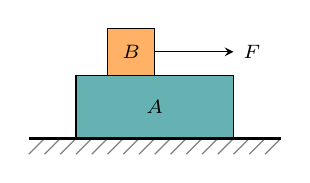
\begin{tikzpicture}[font=\scriptsize]
	\draw[fill=teal!60] (0,0) rectangle(2,.8)node[midway]{\(A\)};
	\draw[fill=orange!60] (.4,.8) rectangle(1,1.4)node[midway]{\(B\)};
	\draw[-stealth] (1,1.1)--++(1,0)node[right]{\(F\)};
	\foreach \x in {-.6,-.4,...,2.6}
		\draw[gray] (\x,-.2)--++(.2,.2);
	\draw[thick] (-.6,0)--(2.6,0);
\end{tikzpicture}
\begin{choices}
	\item \(0.5\mu mg\) 
	\item \(\mu mg\)
	\item \(2\mu mg\)
	\item \(3\mu mg\)
\end{choices}
\begin{answer}
	C\qquad 提示：
\end{answer}